\documentclass[12pt]{report}
\usepackage{xcolor} % for different colour comments
\usepackage{parskip} % Space between each paragraph.
%\usepackage{hardwrap} % for text length of 80 pts
\usepackage[margin=1.2in]{geometry}
\usepackage{hyperref}
\usepackage{../ltx/edcomms}
\usepackage{graphicx}
\usepackage[section]{placeins} % Prevents floats from floating across sections
\usepackage{natbib}%Bibtex
\usepackage{float}
\usepackage{tabularx}
\usepackage{ltablex} %% Multi page tables 
\usepackage{booktabs}
\usepackage{amsfonts}
\usepackage{amssymb}
\usepackage{tabto}
\usepackage{tocloft} %% This package prevents table of contents from generating a page break
\usepackage{caption}
\usepackage{ifthen}
\usepackage{../ltx/edcomms}

%% Comments are enabled and disabled by 'draft' mode. I hacked in my own draft
%% mode (https://en.wikibooks.org/wiki/LaTeX/Macros) because the LaTeX draft
%% mode disables a bunch of things that I don't want it to. I just want it to
%% disable comments. Do not set any of this manually, just use the build script,
%% which builds both draft and final copies. Comments are enabled by default, so
%% if you build manually, you get a draft copy. 
\providecommand\draftmode{true}

\ifthenelse{\equal{\draftmode}{true}}{
\newcommand{\authornote}[3]{\textcolor{#1}{[#3 ---#2]}}
\newcommand{\todo}[1]{\textcolor{red}{[TODO: #1]}}
%\edcommstrue %% Dr. Kahl's comment package. Eventually we should migrate all
             %% comments to this.
}{
\edcommsfalse 
\newcommand{\authornote}[3]{}
\newcommand{\todo}[1]{}
}

% wss = Dr. Smith ; ds = Dr. Szymczak
\newcommand{\wss}[1]{\authornote{magenta}{SS}{#1}}
\newcommand{\ds}[1]{\authornote{blue}{DS}{#1}}


\usepackage{geometry}
\usepackage{changepage}
\setlength{\parindent}{15pt} % parskip sets this to 0. 15 is default.

\newcolumntype{C}[1]{>{\centering}p{#1}} %% For use with tabularx
%%%%%%%%%%%%%%%	START OF DOCUMENT %%%%%%%%%%%%%%%%%%%%
\edcommsfalse
\begin{document}

\pagenumbering{roman} %% Roman numerals before actual document starts
\begin{titlepage}\begin{center}
\thispagestyle{empty} %% No page no. on title

\vspace*{1cm}

{\Huge\textbf{Ampersand Event-Condition-Action Rules}}

\vspace{0.5cm}
{\Large Software Requirement Specification 
	
	\edinsert{JG}{Version 0 Revised}

\vspace{1.5cm}
Yuriy Toporovskyy,\ Yash Sapra,\ Jaeden Guo}
\vfill

We acknowledge that this document uses material from the Volere Requirements
Specification Template, copyright 1995 - 2012 the Atlantic Systems Guild
Limited.

\vspace{0.8cm}
\end{center}
CS 4ZP6 \\
October 9th, 2015 \\ 
Fall 2015 / Winter 2016 
\end{titlepage}

%% Revision history

\begin{table}[ht!]\begin{center}
\caption{Revision History}  
\begin{tabular}{|l|l|l|}\hline
\textbf{Author} & \textbf{Date} & \textbf{Comment} \\\hline 
Yuriy Toporovskyy & 26 / 09 / 2015 & Initial skeleton version \\\hline
Yuriy Toporovskyy & 30 / 09 / 2015 & Project drivers, description and \\ & & 
added project diagram and project flow chart \\\hline
J Guo & 09 / 10 / 2015 & Update: Non-Functional first half 4.1-4.3, added to 
1.2.2, \\ & & completed 2.2 \\\hline
J Guo & 13 / 10 / 2015 & Update: Figures added for Non-Functional 4.1-4.7,  \\ 
& & 
Non-Functional second half 4.4-4.7 half, \\ & & added Functional 3.3 - System 
requirements  and \\ 
& & diagram figure, \& Section 5.8 \\\hline
Yash Sapra &  12/ 09 / 2015 & Non-Functional - legal requirements, \\ & & Functional - User 
Requirements, tasks, risks \\ & & and chapter 5.
\\\hline
Yuriy Toporovskyy & 13 / 10 / 2015 & Initial round of editing \\\hline
J Guo & 04/ 02/ 2016 & Revision 0\\\hline
\end{tabular}
\end{center}\end{table}

\newpage

\tableofcontents
\listoffigures
\listoftables

\newpage
\pagenumbering{arabic} %% Arabic numerals in actual document

%%%%%%%%%%%%%%%%%%%%%%%%%%%%%%%%%%%%
%% Chapter 1: ???                 %%
%%%%%%%%%%%%%%%%%%%%%%%%%%%%%%%%%%%%
\setlength{\arrayrulewidth}{0.35mm}
\setlength{\tabcolsep}{16pt}
\renewcommand{\arraystretch}{2}
\begin{figure}
	\begin{adjustwidth}{-1cm}{}
	\begin{tabular}{ |m{4cm}|m{6cm}|m{4cm}|  }
		\hline
		\multicolumn{3}{|c|}{\bfseries{Project Time Table}} \\
		\hline
		\bfseries{Projected Finish Date}& \bfseries{Milestone} & 
		\bfseries{Actual Finish Date} \\
		\hline
		 09/10/2015& EFA SRS version 0 & 13/10/2015 \\
		19/10/2015 & EFA SRS version 1  & 22/10/2015 \\
		23/10/2015 & Proof of Concept Demonstation & 19/01/2016 \\
		11/02/2016 & Software Demonstration & 11/02/2016 \\
		%%--- & --- & --- \\
		01/04/2016 & EFA Complete & --- \\
		\hline
	\end{tabular}
	\end{adjustwidth}
\end{figure}
\chapter{Ampersand As A System}\label{ch:Intro}

\begin{figure}[!htb]
\centering
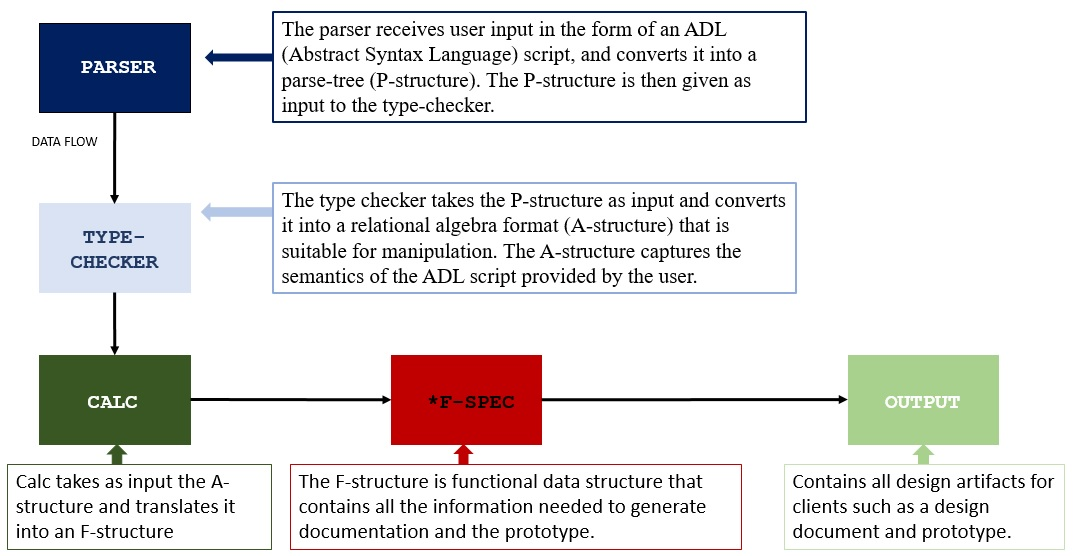
\includegraphics[width=\textwidth]{../figures/ampersand_parts}
\caption{Components of Ampersand System}~\label{fig:AmpersandParts}
\end{figure}

%%
%%\begin{figure}[!htb]
%%	\centering
%%	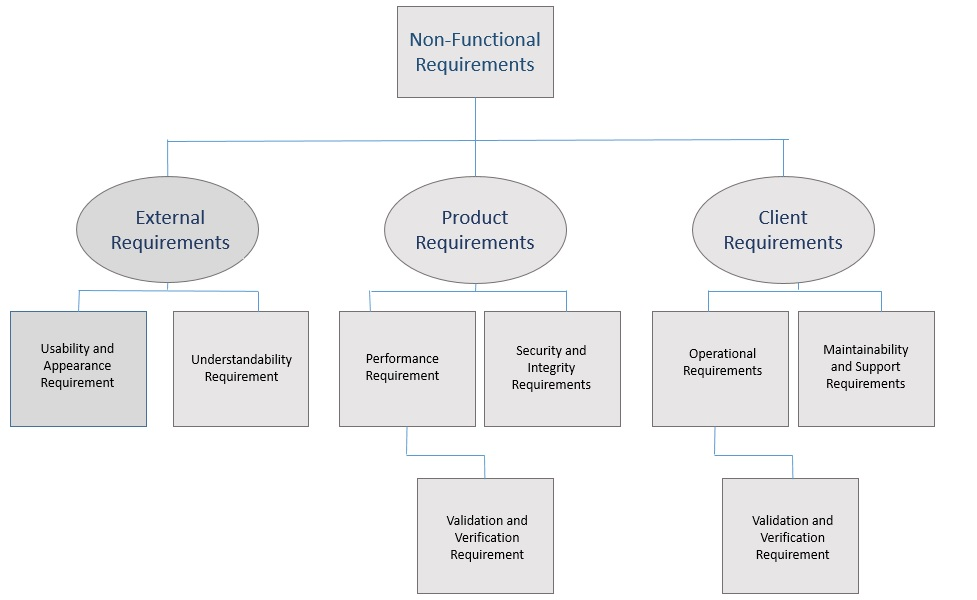
\includegraphics[width=0.8\textwidth]{../figures/NONFUNCTIONAL}
%%	\caption{Tree of non-functional requirements as it relates to EFA}~\label{fig:figure2}
%%\end{figure}
%%
\paragraph{}
Ampersand is an open-source project that produces design artifacts based on 
business rules. One of the essential functions of Ampersand is to maintain all 
the business rules that keep transactions valid during the course of each 
cycle, where multiple transactions could take place.  Figure 1.1  breaks 
down the major components of Ampersand ignoring specification details. This 
project focuses mainly on one component of Ampersand, which is the F-spec which 
contains ECA (Event-Condition-Action Rules) that each process must obey. These 
rules are essential to the functionality of Ampersand, and purpose of this 
project is to correctly translate ECA Rules into type safe SQL queries.
{\section{The Ampersand Environment}\label{sec:Purpose}}
Ampersand is a on-going project with an increasing number of modules being
added to it on a weekly basis. Since this project focuses on a component of 
Ampersand, it must be built to fit within the Ampersand environment and 
co-exist with other modules. Due to this restriction, many design decisions are 
predetermined such as types of data that are used and programming language used 
to build them.
\subsection{Project Purpose}
The purpose of this project is to correctly translate ECA rules
 into type-safe SQL queries using Haskell. These ECA rules are used to 
maintain business constraints.
\subsection{Project Goals} 
The goals of this project can be divided into two components. The first 
component consists of satisfying the condition necessary for the completion of 
an undergraduate capstone project. The second component is to design and 
implement maintainable code that can be absorbed to the Ampersand open-source 
project. 
\section{The Stakeholders}\label{sec:Stakeholders}
The stakeholders are separated into two sections, those that directly benefit 
from this projects contribution and those that indirectly benefit.
\subsection{Ampersand Designers}\label{subsec:Ampersand}
Ampersand designers are our client, and they directly benefit from this project 
as it bring Ampersand one step closer to completion. This project EFA (ECA for 
Ampersand) delivers a maintainable component for Ampersand that produces type 
safe SQL queries, which will be used to maintain the consistency of the data in the back-end Database. 

\subsection{End-Users}\label{subsec:BusReq}
\paragraph{}
Ampersand users indirectly benefit from this project's contribution because it 
drastically decrease the time spent manually restoring system invariants, which 
are the rules that maintain the validity of each business process. As EFA is 
executed during compile time, the user will not suffer any noticeable delays 
and can rest assured that the artifacts they received are correct according to 
specification.

%%%%%%%%%%%%%%%%%%%%%%%%%%%%%%%%%%%%
%% Chapter 2: Project Constraints %%
%%%%%%%%%%%%%%%%%%%%%%%%%%%%%%%%%%%%
\chapter{Project Constraints}\label{ch:Constraints}
The current Ampersand system is the main limitation of this project; everything 
that is built, must be built to fit within its current constraints. These 
constraints include the language used to build Ampersand (i.e. Haskell). 
Anything incorporated into Ampersand must be implemented in the Haskell 
language. An Additional constraint placed on 
the acceptance of this project by our clients is to produce maintainable 
code; this includes the use of dependable libraries and any support modules 
generated by this project to help the translation of ECA rules to SQL queries.

\section{Mandated Constraints}\label{sec:Constraints}
%%%%
%% 4.1 Solution constraints. 

All code must be well documented, backwards compatible and fit seamlessly into 
the current Ampersand project. Due to the long-term nature of this project, we 
must minimize the number of external dependencies. 

%%3b.
\subsection{Implementation Environment of the Current System}
\subsubsection*{Haskell}
The Ampersand code base is written almost entirely in Haskell 
(\cite{ampSource}) with the exception of user interfaces for the generated 
prototypes written in PHP and Javascript. Haskell is the only programming 
language we can use to build modules for Ampersand.


\subsubsection*{The Glasgow Haskell Compiler \& Cabal Build System}
As most of Ampersand's base code is written in Haskell, a compiler must be used 
to compile it. The Glasgow Haskell Compiler (\cite{GHC}) with the Cabal build 
system (see \verb|ampersand.cabal| must be used to compile Ampersand 
\cite{ampSource}). Ampersand is not designed to used with other Haskell 
compilers.


\subsubsection*{GitHub Repository}
Ampersand's main repository is hosted on Github, we must also host our project 
on Github to be able to maintain consistency with the Ampersand source code.

\subsubsection*{Graphviz}
Graphviz is an open source graph visualization software, which can
visually represent information in the form of charts and graphs. Graphviz is 
used to create visuals in Ampersand artifacts and is essential to running 
Ampersand.

%%removed XAMPP, not a constraint

\subsection{Partner of Collaborative Applications}
\edcomm{JG}{3c. of voltere template, applications that are not part of product 
but with which the product will collaborate, can be external applications, 
commercial packages or pre-existing in-house applications}

\begin{longtable}{ |m{4.5cm}|m{1.5cm}|m{7cm}|  }
    \hline 
    \textbf{Name} & \textbf{Type} & \textbf{Description} \\ \hline \hline
    AbstractSyntaxTree & Ampersand module & A module designed specifically for 
    Ampersand, data from this module is manipulated in EFA.
    \\ \hline        
    Control.Applicative & Library module & An interface that provides an 
    intermediate structure between a monad and a functor. This interface is 
    used to embed pure expressions, sequence computations and combine their 
    results.  \\ \hline
    Control.Exception & Library module & An interface that provides support for 
    raising and catching build-in and user-defined exceptions.  \\ \hline
    Control.DeepSeq & Library module & This module is used to fully evaluate 
    data structure and is used to prevent resource leaks in lazy IO programs.  
    \\ \hline            
    Data.Proxy & Library module & A concrete proxy type, used to represent the 
    value of something else.  \\ \hline    
    Data.Type.Equality & Library module & This module offers pattern-matching 
    on types and provides a proof, it is used as a definition of propositional 
    equality.  \\ \hline        
    Data.List & Library module & A module that provides support for operations 
    on list structures.  \\ \hline
    Data.Char & Library module & A module that provides support for characters 
    and operations on characters.  \\ \hline
    Data.Coerce & Library module & Provides safe coercions between data types; 
    allows user to safely convert between values of type that have the same 
    representation with no run-time overhead.   \\ \hline
    Debug.Trace & Library module & Interface for tracing and monitoring 
    execution, used for investigating bugs and other performance issues.  \\ 
    \hline
    GHC.TypeLits & Library module & Internal GHC module that declares the 
    constants used in type-level implementation of natural numbers.  \\ 
    \hline    
    GHC.Exts & Library module & This modules allows the use of pointers to an 
    object or array of objects.  \\ \hline    
    Language.SQL.SimpleSQL & Library module & Syntax: provides the AST for SQL 
    queries. \\& & Pretty: provides pretty printing functions that formates 
    output for human reading. \\ \hline            
    Numeric.Natural & Library module & Natural number type  \\ \hline    
    Prelude & Library module & A standard module that is imported by default 
    and provides support for basic data types, comparison functions, and 
    methods used for data manipulation.   \\ \hline
    System.IO.Unsafe & Library module & This module allows IO computation to be 
    performed at any time, the IO computation must be free of side effecets and 
    independent of its environment to be considered safe. Any I/O computation 
    that is wrapped in unsafePerformIO performs side effects.  \\ \hline
    Text.PrettyPrint.Leijen & Library module & A pretty printer module based 
    off of Philip Wadler's 1997 "A prettier printer", used to show SQL queries 
    in a readable manner to humans.  \\ \hline        
    Unsafe.Coerce & Library module & A helper module that converts a value from 
    any type to any other type, the user must assure that the old data type and 
    the new data type have identical internal representations, else runtime 
    corruption occurs. This is used in the translation of ECA rules to SQL 
    using unique data types.  \\ 
    \hline  
\end{longtable}
\section{Naming Conventions and Terminology}\label{sec:Naming} 
\begin{description}
\item[ECA] Stands for Event-Condition Action. The rule structure used for data
  bases and commonly used in market ready business rule engines. ECA rules are
  used in Ampersand to describe how a database should be modified in response to
  a system constraint becoming untrue.
  
\item [ADL] Stands for ``Abstract Data Language'' (\cite[13]{derFun}). From a
given set of formally defined business requirements, Ampersand generates a
functional specification consisting of a data model, a service catalog, a
formal specification of the services, and a function point analysis. An ADL
script acts as an input for Ampersand. An ADL file consists of a plain ASCII
text file.
\item [Ampersand] Ampersand is a method and the name of the open source 
project. 
    \begin{itemize}
        \item[$\Rightarrow$] The Ampersand method is used to generate
        functional specification from formalized business requirements.
        \item[$\Rightarrow$] The Ampersand software is a tool that implements 
        this method.
    \end{itemize} 
    
\item [Business rules] Rules that exist to represent real world 
constraints that the virtual world does not naturally possess, such as resource 
and social limitations. Examples of constraints include but are not limited to 
financial, logistic, physical or legal constraints.

\item [EFA] Stands for ``ECA (see above) for Ampersand''. This term is used to 
refer to this project. 
\item [Functional specification] A \emph{formal} document which details the 
operation, capabilities, and appearance of a software system. 

\item [Natural language] Language written in a manner similar to that of human 
communication; 
  language intended to be interpreted and understood by humans, as opposed to 
  machines. 
  
\item [Requirements engineering] The process of translating business
requirements into a functional specification. 
\end{description}

\section{Relevant Facts and Assumptions}\label{sec:Assumptions}
This project makes the assumption that Ampersand users are using it according 
to its intended purposes and have all the necessary software dependencies 
installed for it properly function. This project is designed with the 
assumption that no direct interaction is necessary between the design component 
and the user. All interactions that could take place is buffered by Ampersand. 
Furthermore, we assume that Ampersand users are industry professionals that are 
capable of tracing error messages and fixing them. 

\subsection{Error Detection}
EFA provides traceable error messages for the developer, however on a user 
level these trace error messages would be absorbed into Ampersand and its 
various error detection mechanisms situated on every level of compilation. 
Ampersand is equipped with friendly error detection for the user beginning with 
syntax detection for ADL scripts to assure that there are no missing or out of 
place components. To logical error detections that the user might have missed 
during the creation of their information system. The error messages inform the 
user what line the error has been found, what the error pertains to, and what 
is expected typically in the script structure. The script structure provides 
the user clues for how they may wish to fix the error by adjust their script to 
fit the appropriate format.

%%%%%%%%%%%%%%%%%%%%%%%%%%%%%%%%%%%%%%%%%%
%% Chapter 3 -- Functional requirements %%
%%%%%%%%%%%%%%%%%%%%%%%%%%%%%%%%%%%%%%%%%%
\chapter{Functional Requirements}\label{ch:Functional}
\begin{figure}[!htb]
    \begin{center}
        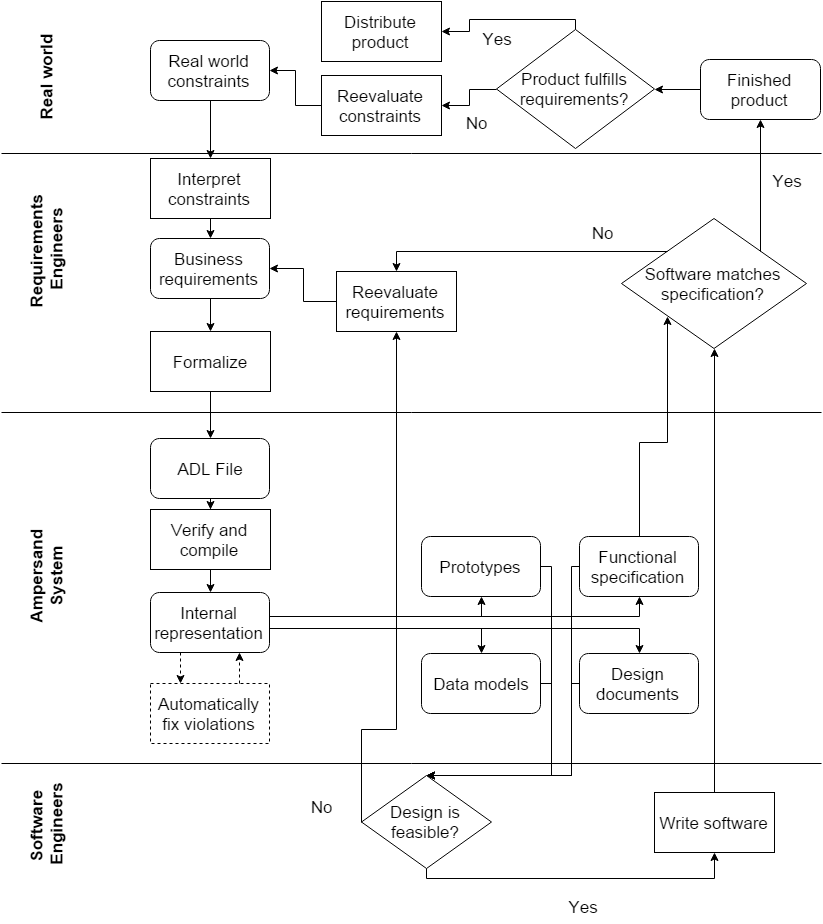
\includegraphics[width=\textwidth]{../figures/business_process}
        \caption{Business process diagram representing the role of Ampersand in 
        the software design cycle}~\label{fig:BusinessProcess} \end{center}
The diagram is a simplified view of the software design cycle, intended to 
highlight 
the role of Ampersand in this cycle. This view omits many of the uses of the 
design artifacts generated by Ampersand; instead it focuses mainly on the 
primary purpose, which is to help create a finished software system. 

The contribution of this project is denoted with dashed lines. Note that it is
isolated to a process completely internal to Ampersand.    
\end{figure}


\section{The Scope of the Work}\label{sec:ScopeOfWork}
\textit{The following sections focuses specifically on EFA and how it will 
function in the Ampersand environment.}
%data flow diagram for EFA goes here
EFA is an automated process internal to Ampersand, and as a part of the 
Ampersand system it works in collaboration with other internal components such 
as the F-spec. The purpose of EFA is to replace the current exec-engine, 
creating a permanent solution for the implementation of ECA rules. EFA also 
provides extensive functionalities that the exec-engine is missing, such as the 
ability to manipulate data in a database beyond the basic level of creating and 
dropping tables, and basic select queries. It provides the fundamental 
datatypes that are crucial for the expansion and maintenance of Ampersand as it 
grows. Due to the way that queries are generated in its present state, large 
number of projects will bog down the system until it becomes unmanageable, and 
if Ampersand is used in practice.

\subsection{The Current Situation} %what is being replaced/made better, the 
%effects of the proposed change

Ampersand currently has an exec-engine that passes SQL queries which are 
triggered by the prototype user interface implemented in PHP. Though the 
exec-engine functions, it is a temporary solution for translating ECA rules 
into SQL queries. Any changes made to the information system after its initial 
generation require manual maintenance. This project will create a permanent 
solution that is provably correct and will automate the correction of system 
invariants so that manual maintenance of system invariants is no longer 
necessary once EFA has been successfully incorporated into Ampersand.

\section{The Scope of the Product}\label{sec:ScopeOfProduct}
The translation of ECA rules into SQL queries require unique data types that 
preserves the semantics the user provides in the ADL script. ECA rules are 
generated from the conditions the user specifies in the ADL script. The SQL 
queries generated from ECA rules can be thought of as a sequence of changes 
made to the data. This sequence of actions are made through specific event 
triggers, and the actions only take place if all conditions are satisfied and 
are valid. An example of this, would be attempting to delete a person who does 
not exist. This actions cannot be completed because the person does not exist, 
this action would be invalid. 

\section{Functional Requirements}\label{sec:Functional}
\ds{What about error handling on the new contributions?
    Where's the functional requirement related to: 
    ``be a pure function; it should not have side effects." and 
    ``provide diagnostic information about the algorithm to
    the user, if the user asks for such information."?}

\subsection{System Requirements}
%%-----------------------------SIDE EFFECTS---------------------------------%%
{\setlength{\tabcolsep}{6pt} %% Default is 6
    \begin{tabularx}{\textwidth}{>{\bfseries}m{3cm}X}
        Requirement & S1 \\ 
        \midrule
        \endhead
        Description  & Create pure functions with no unintended side effects
        \\	Rationale & The use of a functional programing languages requires 
        that this program be a pure function and does not have side effects, 
        however certain portions of the code requires the execution of side 
        effects to match the behaviour presented by external programs. In these 
        specific instances, the side effects are an intended behaviour.
        \\	Originator & Stakeholder/Developer
        
        \\	Fit Criterion & This behaviour is necessary to produce the results 
        the stakeholders desire
        \\ Test Case & Desired results can be confirmed as they will be 
        reflected in changes that take place in the Ampersand database.
        \\	Customer Satisfaction & 5 - Highest 
        \\	Priority & 5 - Highest 
        \\	Supporting Materials & (Rule Based Design \cite {RBD})
        \vspace{12pt}
    \end{tabularx}
}

%%------------------USE OF HASKELL AS IMPLEMENTATION LANGAUGE-----------------%%
{\setlength{\tabcolsep}{6pt} %% Default is 6
    \begin{tabularx}{\textwidth}{>{\bfseries}m{3cm}X}
        Requirement & S2 \\ 
        \midrule
        \endhead
        Description  & The use of Haskell to implement EFA modules
        \\	Rationale & The source code of Ampersand is written completely in 
        Haskell, and thus Haskell must be used for any modules created by this 
        project to be absorbed into the pre-existing source code.
        \\	Originator & Ampersand Creators (i.e. our client)        
        \\	Fit Criterion & Primary ability to write code compatible with 
        Ampersand as it is.
        \\ Test case & Added modules are tested with cabal build inside of 
        Ampersand
        \\	Customer Satisfaction & 5 - Highest 
        \\	Priority & 5 - Highest 
        \\	Supporting Materials & Dr. Joosten, Joosten and Kahl
        \vspace{12pt}
    \end{tabularx}
}
%%------------------ MODULES MUST FIT AMPERSAND FRAMEWORK-----------------%%
{\setlength{\tabcolsep}{6pt} %% Default is 6
    \begin{tabularx}{\textwidth}{>{\bfseries}m{3cm}X}
        Requirement & S3 \\ 
        \midrule
        \endhead
        Description  & Added modules must fit within Ampersand's current 
        framework
        \\	Rationale & As Ampersand is a huge system that has weekly additions 
        to prevent conflict and breaking of existing packages/modules, an 
        effort should be made to minimize external dependencies. As EFA will be 
        an internal component of Ampersand, if a package that EFA depends on to 
        function properly is no longer maintained and breaks, it will in turn 
        break Ampersand.
        \\	Originator & Ampersand Creators (i.e. our client)        
        \\	Fit Criterion & Functionality of EFA as an Ampersand internal 
        component.
        \\ Test case & Added modules are tested with cabal build inside of the
        Ampersand system as an internal component (i.e. System testing)
        \\	Customer Satisfaction & 4 - High 
        \\	Priority & 4 - High
        \\	Supporting Materials & Hackage, Dr. Kahl
        \vspace{12pt}
    \end{tabularx}
}
%%----------------------- MACHINE--------------------------------------------%%
{\setlength{\tabcolsep}{6pt} %% Default is 6
    \begin{tabularx}{\textwidth}{>{\bfseries}m{3cm}X}
        Requirement & S4 \\ 
        \midrule
        \endhead
        Description  & Machine-checked proofs
        \\	Rationale & EVA data-types are indexed on Haskell types, and 
        indices are selected in a way that impossible values are eliminated by 
        Haskell's strong type system.
        \\	Originator & Stakeholder/Developer
        
        \\	Fit Criterion & Program compiles and provides an inductive proof 
        that the SQL generated by ECA2SQL is correct
        \\ Test Case & Verified by examination
        \\	Customer Satisfaction & 5 - Highest 
        \\	Priority & 5 - Highest 
        \\	Supporting Materials & Requirement solicitation.
        \vspace{12pt}
    \end{tabularx}
}
\subsection{Project Requirements}
%%-------------------------TYPE CORRECTNESS ----------------------------------%%
{\setlength{\tabcolsep}{6pt} %% Default is 6
    \begin{tabularx}{\textwidth}{>{\bfseries}C{3cm}X}
        Requirement & P1 \\ 
        \midrule
        \endhead
        Description  & Provable Correctness: Haskell like other functional 
        programming languages have 
        a strong type system which can be used for machine-checked proofs.
        \\	Rationale & Curry-Howard correspondence which states that the 
        return type of the function is analogous to a logical theorem, that is 
        subject to the hypothesis corresponding to the types of the argument 
        values that are passed to the function and thus the program uysed to 
        compute that function is analogous to a proof of that theorem.
        \\	Fit Criterion & Provable correctness of the program that is 
        generated.
        \\ Test Cases & Internal structure of ECA rules can be compared to SQL 
        queries through a series of datatype tests, each of which will result 
        in a traceable result or error message
        \\	Priority & 4 - High
        \\	Supporting Materials & Programming language theory, Dr. Kahl
        \vspace{12pt}
    \end{tabularx}
}
%%--------------------------CORRECTNESS OF ECA TO SQL RULES ------------------%%
{\setlength{\tabcolsep}{6pt} %% Default is 6
    \begin{tabularx}{\textwidth}{>{\bfseries}C{3cm}X}
        Requirement & P2 \\ 
        \midrule
        \endhead
        Description  & Generated SQL queries must preserve the semantics of ECA 
        rules.  
        \\	Rationale & The translation would otherwise not be correct, as the 
        rules would be meaningless if their semantics are lost.
        \\	Originator & Ampersand Developers
        \\	Fit Criterion & Generated queries must be provably correct as per 
        client's request.
        \\ Test Cases & Internal structure of ECA rules can be compared to SQL 
        queries through a series of datatype tests, each of which will result 
        in a traceable result or error message
        \\	Priority & 4 - High
        \\	Supporting Materials & Hackage, Dr. Kahl
        \vspace{12pt}
    \end{tabularx}
}
%%-------------------------TRACABLE EERRORS---------------------------%%
{\setlength{\tabcolsep}{6pt} %% Default is 6
    \begin{tabularx}{\textwidth}{>{\bfseries}C{3cm}X}
        Requirement & P3 \\ 
        \midrule
        \endhead
        Description  & Generating traceable results and error messages for 
        handling new contributions from this project
        \\	Rationale & Saves time by allowing the program to inform the 
        programmer where the errors are located.
        \\	Originator & Ampersand Developers
        \\	Fit Criterion & Errors must be traceable and have a standard format 
        that can be easily followed.
        \\ Test Cases & Error message will print to screen.
        \\	Priority & 4 - High
        \\	Supporting Materials & Hackage, Dr. Kahl
        \vspace{12pt}
    \end{tabularx}
}

\subsection{Non-Functional Requirements}
%%---------------------------AVAILABILITY TO USERS REQUIREMENT ---------------%%
{\setlength{\tabcolsep}{6pt} %% Default is 6
\begin{tabularx}{\textwidth}{>{\bfseries}C{3cm}X}
Requirement & N1 \\ 
\midrule
\endhead
Description  & EFA must be available at anytime Ampersand is running.
\\	Rationale & To provide the user with unlimited access to EFA within 
Ampersand.
\\	Originator & Ampersand Developers
\\	Fit Criterion & Ampersand can detect when internal components are 
non-responsive
\\ Test cases & Ampersand is subject to sentential tests on a daily basis as 
part of its maintenance.   
\\	Priority & 4 - High
\\	Supporting Materials & Useful feedback in Ampersand parser \cite{SB2011}
\vspace{12pt}
\end{tabularx}
}


\chapter{Non-Functional Requirements}\label{ch:NonFunc}
\begin{figure}[!htb]
	\centering
	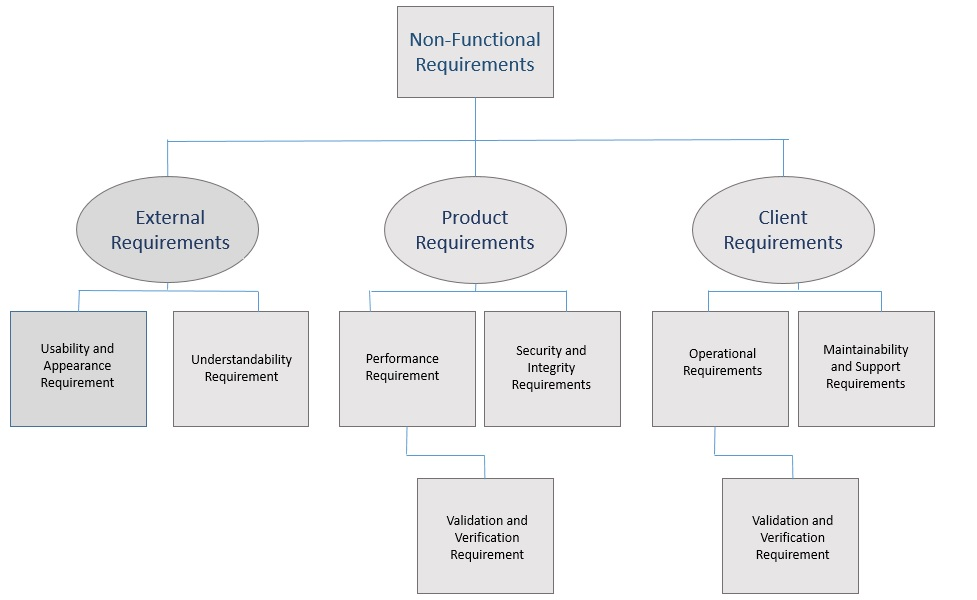
\includegraphics[width=0.8\textwidth]{../figures/NONFUNCTIONAL}
	\caption{Tree of non-functional requirements as it relates to 
	EFA}~\label{fig:figure2} 
\end{figure}
    Each Non-functional requirement must be traceable in the Ampersand system 
    with the addition of EFA. 
    \textit{Note: Missing sections in this chapter are not applicable for this 
    project }
\section{Performance Requirements}\label{sec:Performance}
\paragraph*{}
EFA is designed to optimize the Ampersand system by automating the tedious task 
of restoring system invariants when broken using ECA rules. Ampersand will 
perform as it use to with less maintenance required on behalf of the user.
\section{Maintainability and Support Requirements}\label{sec:Support}
\paragraph*{}
EFA must make sure that each specification/error is traceable 
(\cite[2]{derFun}). EFA will be upgrade and tested as a part of Ampersand does 
not require additional maintenance or support to perform optimally.

\section{Validation and Verification Requirements}\label{sec:Verification}


\begin{longtable}{|m{5cm}|m{9cm}| }
    \hline 
    \textbf{Notation}  & \textbf{Description} \\ \hline
       X : Y   &  X has type Y \\ 
        \hline  
       $`Types`$  &  Type of types \\ 
        \hline
       $`Kind`$   &  Type of Kinds \\ 
        \hline
         \_ $\rightarrow$ \_ ∶ Type →$\rightarrow$Type $\rightarrow$ Type  & 
         This function requires 2 Type inputs and produces a Type output. Where 
         \_ $\rightarrow$ \_ can be seen as for each element x of type A 
         defines a function F(x) where x does not exist in set {Type,Kind} for 
         every x that defines F(x)  \\ 
        \hline
       \_ $\rightarrow$ \_∶ Kind $\rightarrow$Kind $\rightarrow$ Kind  & This 
       function requires 2 of type Kinds and produces an output of Type Kinds . 
       Where 
       \_ $\rightarrow$ \_ can be seen as for each element x of type A 
       defines a function F(x) where x does not exist in set {Type,Kind} for 
       every x that defines F(x). This a dependent type, an example of this 
       would be 
       SingT (x :: a) $\rightarrow$ SingT (F x)
       \\ 
        \hline
          $\mathbb{N}$, Symbol : Kind   &  Left of the : are the elements that 
          represent type Kinds (right of the : )\\ 
        \hline
          0, 1, 2, $...$ ∶ $\mathbb{N}$   &  These are natural numbers, 
          elements left of the : belong to the set N of natural numbers\\ 
        \hline
         \{$""$, $"a"$, $"aa"$, $...$, $"b"$, $"bb"$\} : Symbol &  
         Elements left of : are elements that belong to the set Symbol \\ 
        \hline
        ( x : A  ) $\rightarrow$ F x   & \\ where x $\notin$ \{Type,Kind\}   &  
        This can also be seen as $\forall$ x $\rightarrow$ F x; where as  \\ 
        \hline
           SingT \(x $::$ a\) $\rightarrow$ SingT \(F x\)  &  SingT is the type 
           of singleton, a dependent type created for EFA datatypes. \\ 
        \hline
          $\rightarrow$: Constraint $\rightarrow$ Type $\rightarrow$ Type  and  
          \_ $\Rightarrow$ \_ : Type $\rightarrow$ Constraint $\rightarrow$ 
          Type    &  where $\forall$x : S $\Rightarrow$ T corresponds to 
          $\mathbf{G}$ \textit{S} ($\lambda$x.T) in Illative Combinatory 
          Logic 
          where G is the combinator \cite{CombLogic}. The $\Rightarrow$ 
          represents restraints for what on the right side of the : .\\ 
        \hline
        X : Y  where Y $\in$ {Type,Kind} &  X is equal in definition to 'X : 'Y 
        and only X' : Y'. \\ 
        \hline
        elim-Y: (r:Type) $\rightarrow$ Y $\rightarrow$ ($A_0$ $\rightarrow$ r) 
        $\rightarrow$ ($A_1$ $\rightarrow$ r ) $\rightarrow$ $\rightarrow$ 
        $...$ $\rightarrow$ ($A_n$ $\rightarrow$ r) $\rightarrow$ r   &  An 
        eliminator that corresponds to pattern matching \\ 
        \hline
        'P : Y $\rightarrow$ Z'   &  This represents 'P (Ctr x)', where 'Ctr  
        is used for type casting\\ 
        \hline
         $\exists$ (x : A) (P x) & This indicates that (r:Type) $\rightarrow$ 
         ((x:A) . (P x $\rightarrow$ r) $\rightarrow$ r) \\ 
        \hline
        X : Y   &  X has type Y \\ 
        \hline
        
\end{longtable}

\section{Module Decomposition}
\textit{Note: * represents the top level module}
\begin{figure}[!htb]
    \centering
    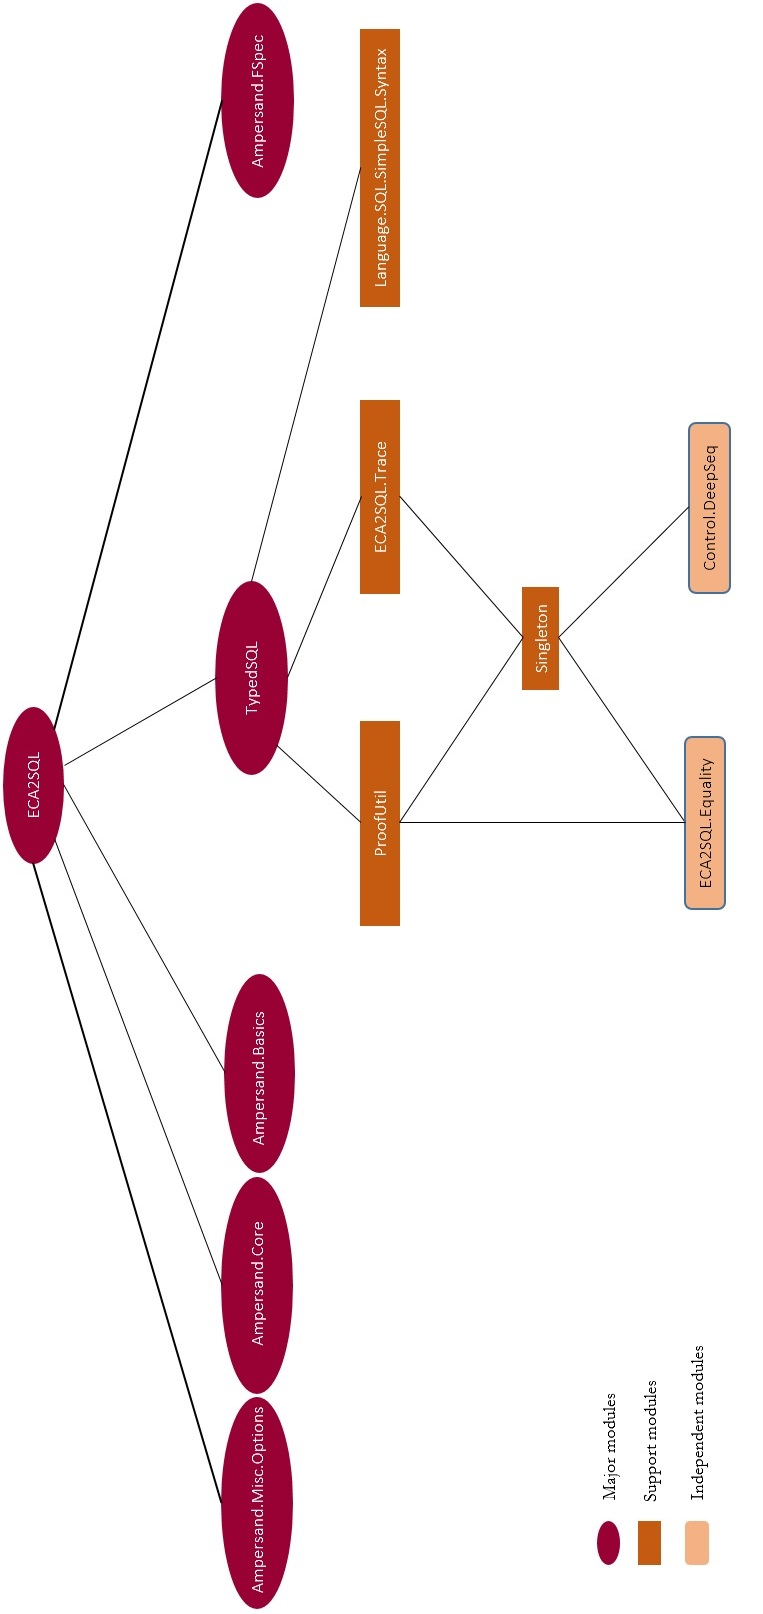
\includegraphics[width=0.65\textwidth]{../figures/projTree}
    \caption{Hierarchy of EFA Modules
        EFA}~\label{fig:figure2} 
\end{figure}

\newpage
\setlength\LTleft{-1in}
\setlength\LTright{-1in}
\begin{longtable}{|m{1.5cm}|m{2.5cm}|m{6cm}|m{6cm}|} \hline
 \textbf{Module}  & \textbf{Functions} &\textbf{Function Types} & 
 \textbf{Description} \\ \hline \hline
    ECA2SQL  & eca2SQL  & Options $\rightarrow$ FSpec $\rightarrow$ ECArule 
    $\rightarrow$ SQLMethod '[] 'SQLBool & d \\ 
    \hline
    ECA2SQL  & eca2PrettySQL  &  Options $\rightarrow$ FSpec $\rightarrow$ 
    ECArule $\rightarrow$ Doc  & d \\ 
    \hline \hline
    a  & b  & c & d \\ 
    \hline
    a  & b  & c & d \\ 
    \hline
    a  & b  & c & d \\ 
    \hline
    a  & b  & c & d \\ 
    \hline
    a  & b  & c & d \\ 
    \hline
    a  & b  & c & d \\ 
    \hline
    a  & b  & c & d \\ 
    \hline
    a  & b  & c & d \\ 
    \hline
    a  & b  & c & d \\ 
    \hline
\end{longtable}
%%%%%%%%%%%%%%%%%%%%%%%%%%%%%%%%%%%%%%%%%%%%%%%%%%%%%
\chapter{Project Issues}\label{ch:issues}
\vspace{-1cm}
\textit{Sections not applicable to this project have been removed}

\section{Tasks}\label{sec:Tasks}
\begin{itemize}
\item Translate ECA rules to SQL commands
\item Create supporting data structures for sustainable translation and future 
maintenance
\item Implement the solution and provide the  annotated source code to the supervisor and the product owner for a review.
\item Incorporate changes to project as suggested by our client and supervisor
\item Provide provable correctness for program
\end{itemize}
\edcomm{YS}{Add in any significant task you feel is worth mentioning}%
\section{Migration to the New Product}\label{sec:Migration}
\paragraph*{}
Upon final review by the client and intensive testing, if the client is
satisfied by the quality of code and its maintainability, the implementation
will be made part of the production stream hosted on Github.  
\section{Risks}\label{sec:Risks}
\begin{itemize}
\item The new code must not introduce any errors or performance regressions
into Ampersand.
\item The code must satisfy existing tests and additional tests written for the 
new algorithm being implemented.
%%I'm pretty sure more goes here
\end{itemize}

\section{Costs}\label{sec:Costs}
\paragraph*{}
The cost is eight months of time.

\section{User Documentation and Training}\label{sec:UserDoc}
\paragraph*{}
User documentation is not necessary, as EFA provides traceable error messages 
for developers. 


\bibliographystyle{alpha}
\bibliography{SRS}
\end{document}










